\section{Tratamento Algébrico}

\subsection{Vetores no Plano}

\begin{figure}[H]
  \centering
  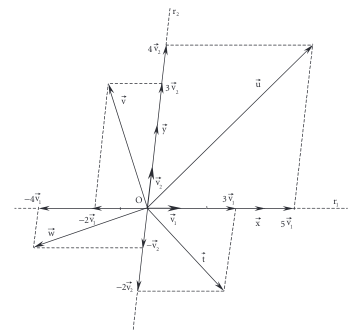
\includegraphics[width=0.6\textwidth]{./fig/fig1.38.png}
  \caption{Vetores expressos em $\vec{v_1}$ e $\vec{v_2}$}\label{fig:fig1.38}
\end{figure}

Na Figura~\ref{fig:fig1.38}, os vetores são combinações lineares de $\vec{v_1}$
e $\vec{v_2}$:

\[
\begin{cases}
  \vec{u} = 5\vec{v_1} + 4\vec{v_2} \\
  \vec{v} = 2\vec{v_1} - 3\vec{v_2} \\
  \vec{w} = -4\vec{v_1} - 3\vec{v_2} \\
  \vec{t} = \vec{v_1} + 2\vec{v_2} \\
  \vec{x} = 3\vec{v_1} - 2\vec{v_2} \\
  \vec{y} = 4\vec{v_2} \\
\end{cases}
\]

\begin{figure}[H]
  \centering
  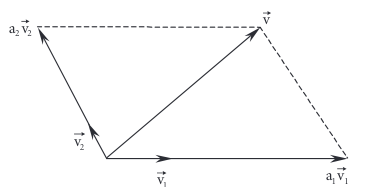
\includegraphics[width=0.6\textwidth]{./fig/fig1.39.png}
  \caption{Representação vetorial no plano}\label{fig:fig1.39}
\end{figure}

Para quaisquer $\vec{v}_1$ e $\vec{v}_2$ não paralelos
(Figura~\ref{fig:fig1.39}), todo vetor $\vec{v}$ do plano pode ser expresso
como:

\begin{equation}\label{eq:combinacao-linear}
  \vec{v} = a_1\vec{v_1} + a_2\vec{v_2}
\end{equation}

O conjunto $\mathcal{B} = \{\vec{v}_1, \vec{v}_2\}$ forma uma base, onde
$(a_1,a_2)_\mathcal{B}$ são as coordenadas de $\vec{v}$. Bases ortonormais
satisfazem $\vec{e}_1 \perp \vec{e}_2$ com $\|\vec{e}_i\|=1$.

\begin{figure}[H]
  \centering
  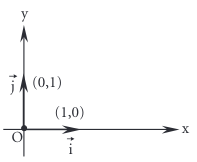
\includegraphics[width=0.4\textwidth]{./fig/fig1.40.png}
  \caption{Base canônica}\label{fig:fig1.40}
\end{figure}

A base canônica $\mathcal{C} = \{\vec{i}=(1,0), \vec{j}=(0,1)\}$
(Figura~\ref{fig:fig1.40}) permite expressar qualquer vetor como:

\begin{equation}\label{eq:combinacao-linear-base-canonica}
  \vec{v} = x\vec{i} + y\vec{j} = (x,y)
\end{equation}

\newpage
\begin{figure}[H]
  \centering
  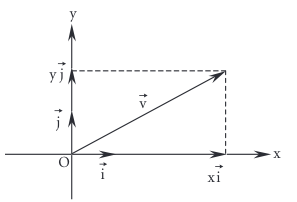
\includegraphics[width=0.5\textwidth]{./fig/fig1.41.png}
  \caption{Vetor no plano cartesiano}\label{fig:fig1.41}
\end{figure}

Na Figura~\ref{fig:fig1.41}, $x$ é a abscissa e $y$ a ordenada de $\vec{v}$.
Exemplos notáveis:

\begin{align*}
  3\vec{i} - 5\vec{j} &= (3, -5) \\
  3\vec{j} &= (0, 3) \\
  -4\vec{i} &= (-4, 0) \\
  \vec{0} &= (0, 0) \\
\end{align*}

\subsection{Igualdade de Vetores}

Dois vetores $\vec{u} = (x_1, y_1)$ e $\vec{v} = (x_2, y_2)$ são iguais se, e
somente se, $x_1 = x_2$ e $y_1 = y_2$, escrevendo-se $\vec{u} = \vec{v}$.

Por exemplo: o vetor $\vec{u} = (x + 1, 4)$ é igual ao vetor $\vec{v} = (5, 2y -
6)$ se

\[
x + 1 = 5 \quad \text{e} \quad 2y - 6 = 4
\] 

ou equivalentemente,

\[
x = 4 \quad \text{e} \quad y = 5
\] 

Assim, se $\vec{u} = \vec{v}$, então $x = 4$, $y = 5$ e $\vec{u} = \vec{v} = (5,
4)$.

\newpage
\subsection{Operações com Vetores}

Para vetores $\vec{u} = (x_1,y_1)$, $\vec{v} = (x_2,y_2)$ e $\alpha \in
\mathbb{R}$, definem-se:

\begin{enumerate}
  \item \textbf{Adição}: $\vec{u}+\vec{v}=(x_1+x_2,y_1+y_2)$
  \item \textbf{Multiplicação por escalar}: $\alpha\vec{u}=(\alpha x_1,\alpha y_1)$
\end{enumerate}

\begin{figure}[H]
  \centering
  \begin{minipage}{0.45\textwidth}
    \centering
    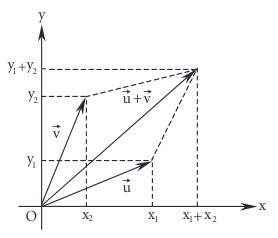
\includegraphics[width=\linewidth]{./fig/fig1.43a.png}
    \caption{Adição vetorial}\label{fig:fig1.43a}
  \end{minipage}
  \hfill
  \begin{minipage}{0.45\textwidth}
    \centering
    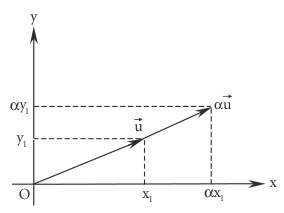
\includegraphics[width=\linewidth]{./fig/fig1.43b.png}
    \caption{Multiplicação por escalar}\label{fig:fig1.43b}
  \end{minipage}
\end{figure}

\noindent\textbf{Operações derivadas}:
\begin{align*}
  -\vec{u} &= (-x_1,-y_1) \\
  \vec{u}-\vec{v} &= (x_1-x_2,y_1-y_2)
\end{align*}

\noindent\textbf{Propriedades}:

\textbf{a)} Álgebra vetorial:
\begin{itemize}
  \item Comutativa: $\vec{u}+\vec{v}=\vec{v}+\vec{u}$
  \item Associativa: $(\vec{u}+\vec{v})+\vec{w}=\vec{u}+(\vec{v}+\vec{w})$
  \item Elemento neutro: $\vec{u}+\vec{0}=\vec{u}$
  \item Inverso aditivo: $\vec{u}+(-\vec{u})=\vec{0}$
\end{itemize}

\textbf{b)} Propriedades mistas:
\begin{itemize}
  \item $\alpha(\beta\vec{v})=(\alpha\beta)\vec{v}$
  \item $(\alpha+\beta)\vec{u}=\alpha\vec{u}+\beta\vec{u}$
  \item $\alpha(\vec{u}+\vec{v})=\alpha\vec{u}+\alpha\vec{v}$
  \item Identidade: $1\vec{v}=\vec{v}$
\end{itemize}

\newpage
\question{Demonstre todas as propriedades listadas.}

\textbf{Álgebra vetorial:}

\begin{compactenum}
  \subquestion{Comutativa: $\vec{u} + \vec{v} = \vec{v} + \vec{u}$}
  \answer{
    A adição de vetores é definida componente a componente. Como a adição de
    números reais é comutativa, temos:
    \[
      \vec{u} + \vec{v} = (u_1 + v_1, u_2 + v_2, \dots, u_n + v_n) = (v_1 + u_1,
      v_2 + u_2, \dots, v_n + u_n) = \vec{v} + \vec{u}.
    \]
  }

  \subquestion{Associativa: $(\vec{u} + \vec{v}) + \vec{w} = \vec{u} + (\vec{v}
  + \vec{w})$}
  \answer{
    Pela associatividade da adição de números reais:
    \[
      (\vec{u} + \vec{v}) + \vec{w} = (u_1 + v_1, \dots, u_n + v_n) + (w_1,
      \dots, w_n) = (u_1 + v_1 + w_1, \dots, u_n + v_n + w_n)
    \]
    \[
      = (u_1 + (v_1 + w_1), \dots, u_n + (v_n + w_n)) = \vec{u} + (\vec{v} +
      \vec{w}).
    \]
  }

  \subquestion{Elemento neutro: $\vec{u} + \vec{0} = \vec{u}$}
  \answer{
    O vetor nulo $\vec{0} = (0, 0, \dots, 0)$ satisfaz:
    \[
      \vec{u} + \vec{0} = (u_1 + 0, u_2 + 0, \dots, u_n + 0) = (u_1, u_2, \dots,
      u_n) = \vec{u}.
    \]
  }

  \subquestion{Inverso aditivo: $\vec{u} + (-\vec{u}) = \vec{0}$}
  \answer{
    O inverso aditivo $-\vec{u} = (-u_1, -u_2, \dots, -u_n)$ satisfaz:
    \[
      \vec{u} + (-\vec{u}) = (u_1 - u_1, u_2 - u_2, \dots, u_n - u_n) = (0, 0,
      \dots, 0) = \vec{0}.
    \]
  }
\end{compactenum}

\textbf{Propriedades mistas:}

\begin{compactenum}
  \subquestion{Associatividade escalar: $\alpha(\beta\vec{v}) =
  (\alpha\beta)\vec{v}$}
  \answer{
    A multiplicação escalar é definida componente a componente:
    \[
      \alpha(\beta\vec{v}) = \alpha(\beta v_1, \beta v_2, \dots, \beta v_n) =
      (\alpha\beta v_1, \alpha\beta v_2, \dots, \alpha\beta v_n) =
      (\alpha\beta)\vec{v}.
    \]
    }

  \subquestion{Distributiva de escalares: $(\alpha + \beta)\vec{u} =
  \alpha\vec{u} + \beta\vec{u}$}
  \answer{
    Pela distributividade dos números reais:
    \[
      (\alpha + \beta)\vec{u} = ((\alpha + \beta)u_1, \dots, (\alpha +
      \beta)u_n) = (\alpha u_1 + \beta u_1, \dots, \alpha u_n + \beta u_n) =
      \alpha\vec{u} + \beta\vec{u}.
    \]
  }

  \subquestion{Distributiva de vetores: $\alpha(\vec{u} + \vec{v}) =
  \alpha\vec{u} + \alpha\vec{v}$}
  \answer{
    Pela distributividade dos números reais:
    \[
      \alpha(\vec{u} + \vec{v}) = \alpha(u_1 + v_1, \dots, u_n + v_n) = (\alpha
      u_1 + \alpha v_1, \dots, \alpha u_n + \alpha v_n) = \alpha\vec{u} +
      \alpha\vec{v}.
    \]
  }

  \subquestion{Identidade escalar: $1\vec{v} = \vec{v}$}
  \answer{
    O número $1$ é o elemento neutro da multiplicação:
    \[
      1\vec{v} = (1 \cdot v_1, 1 \cdot v_2, \dots, 1 \cdot v_n) = (v_1, v_2,
      \dots, v_n) = \vec{v}.
    \]
  }
\end{compactenum}

\newpage
\subsection{Vetor Defnido por Dois Pontos}

Dados os pontos $A(x_1,y_1)$ e $B(x_2,y_2)$, o vetor $\overrightarrow{AB}$ tem
expressão analítica:
\[
  \overrightarrow{AB} = B - A = (x_2 - x_1, y_2 - y_1)
\]

\begin{figure}[H]
  \centering
  \begin{minipage}{0.45\textwidth}
    \centering
    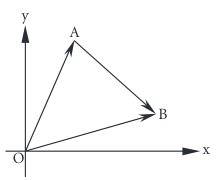
\includegraphics[width=\linewidth]{./fig/fig1.44.png}
    \caption{Vetor $\overrightarrow{AB}$}\label{fig:fig1.44}
  \end{minipage}
  \hfill
  \begin{minipage}{0.45\textwidth}
    \centering
    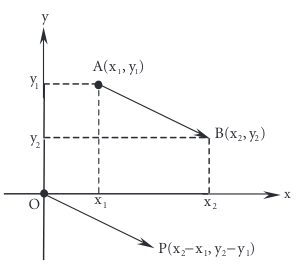
\includegraphics[width=\linewidth]{./fig/fig1.45.png}
    \caption{Representante canônico}\label{fig:fig1.45}
  \end{minipage}
\end{figure}

O representante canônico $\overrightarrow{OP}$ em $O(0,0)$ é o vetor posição que
melhor caracteriza $\overrightarrow{AB}$.

\begin{figure}[H]
  \centering
  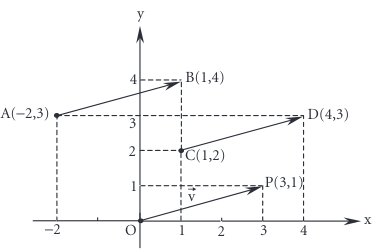
\includegraphics[width=0.6\textwidth]{./fig/fig1.46.png}
  \caption{Equivalência de vetores}\label{fig:fig1.46}
\end{figure}

Na Figura~\ref{fig:fig1.46}, $\overrightarrow{OP}$, $\overrightarrow{AB}$ e
$\overrightarrow{CD}$ representam o mesmo vetor $\vec{v}=(3,1)$, mostrando que a
posição é irrelevante - importam apenas magnitude, direção e sentido.

\newpage
\textbf{Relações importantes}:
\begin{itemize}
  \item $B = A + \overrightarrow{AB}$
    \begin{align*}
      B &= (-2,3) + (3,1) = (1,4) \\
      D &= (1,2) + (3,1) = (4,3) \\
      P &= (0,0) + (3,1) = (3,1) \\
    \end{align*}

  \item Para o triângulo na Figura~\ref{fig:fig1.47}:
    \begin{align*}
      \vec{u} &= \overrightarrow{AB} = (1,2) \\
      \vec{v} &= \overrightarrow{BC} = (-2,2) \\
      \vec{w} &= \overrightarrow{CA} = (1,-4) \\
      \vec{u}+\vec{v}+\vec{w} &= \vec{0} \\
    \end{align*}
\end{itemize}

\begin{figure}[H]
  \centering
  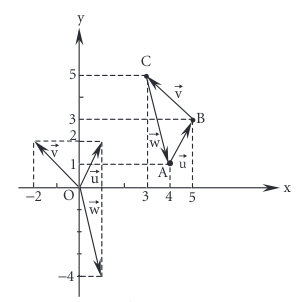
\includegraphics[width=0.4\textwidth]{./fig/fig1.47.png}
  \caption{Vetores em triângulo}\label{fig:fig1.47}
\end{figure}

\newpage
\subsection{Ponto Médio}

Seja o segmento de extremos $A(x_1, y_1)$ e $B(x_2, y_2)$
(Figura~\ref{fig:fig1.50}). Sendo $M(x, y)$ o ponto médio de $AB$, podemos
expressar de forma vetorial como:

\[
  \overrightarrow{AM} = \overrightarrow{MB}
\]

ou

\[
  (x - x_1, y - y_1) = (x_2 - x, y_2 - y)
\]

então

\[
  x - x_1 = x_2 - x \quad \text{e} \quad y - y_1 = y_2 - y
\]

Resolvendo em relação a $x$ e $y$, temos:

\[
  2x = x_1 + x_2 \quad \text{e} \quad 2y = y_1 + y_2
\]

ou

\[
  x = \frac{x_1 + x_2}{2} \quad \text{e} \quad y = \frac{y_1 + y_2}{2}
\]

Portanto,

\[
  M\left(\frac{x_1 + x_2}{2}, \frac{y_1 + y_2}{2}\right)
\]

\begin{figure}[H]
  \centering
  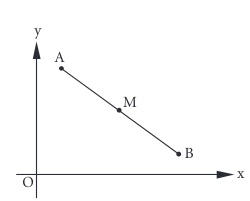
\includegraphics[width=0.5\textwidth]{./fig/fig1.50.png}
  \caption{Ponto médio de um segmento}\label{fig:fig1.50}
\end{figure}

\newpage
\subsection{Paralelismo de Dois Vetores}

Vimos que, se dois vetores $\vec{u} = (x_1, y_1)$ e $\vec{v} = (x_2, y_2)$ são
paralelos, existe um número real $\alpha$ tal que $\vec{u} = \alpha\vec{v}$, ou
seja,

\[
  (x_1, y_1) = \alpha(x_2, y_2)
\]

ou

\[
  (x_1, y_1) = (\alpha x_2, \alpha y_2)
\]

que pela condição de igualdade resulta em

\[
  x_1 = \alpha x_2 \quad \text{e} \quad y_1 = \alpha y_2
\]

donde

\[
  \frac{x_1}{x_2} = \frac{y_1}{y_2} = \alpha
\]

Essa é a condição de paralelismo de dois vetores, ou seja, dois vetores são
paralelos quando suas componentes forem proporcionais.

\subsection{Módulo de um Vetor}

Seja o vetor $\vec{v} = (x, y)$ (Figura~\ref{fig:fig1.51}). Pelo teorema de
Pitágoras, vem:

\[
 |\vec{v}| = \sqrt{x^2 + y^2}
\]

\begin{figure}[H]
  \centering
  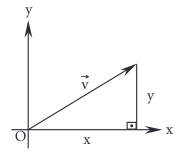
\includegraphics[width=0.4\textwidth]{./fig/fig1.51.png}
  \caption{Módulo de um vetor}\label{fig:fig1.51}
\end{figure}

\textbf{Exemplo}: Se $\vec{v} = (2, -3)$, então:

\[
  |\vec{v}| = \sqrt{(2)^2 + (-3)^2} = \sqrt{4 + 9} = \sqrt{13} \text{ u.c.
  (unidades de comprimento)}
\]

\subsection{Distância entre dois pontos}

A distância entre dois pontos $A(x_1, y_1)$ e $B(x_2, y_2)$
(Figura~\ref{fig:fig1.52}) é o comprimento (módulo) do vetor
$\overrightarrow{AB}$, isto é:

\[
  d(A, B) = |\overrightarrow{AB}|
\]

\begin{figure}[H]
  \centering
  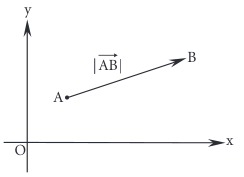
\includegraphics[width=0.5\textwidth]{./fig/fig1.52.png}
  \caption{Distância entre pontos}\label{fig:fig1.52}
\end{figure}

Como $\overrightarrow{AB} = B - A = (x_2 - x_1, y_2 - y_1)$, temos:

\[
  d(A, B) = \sqrt{(x_2 - x_1)^2 + (y_2 - y_1)^2}
\]

\textbf{Exemplo}: Se $A(1, 2)$ e $B(4, 6)$, então:

\[
  d(A, B) = \sqrt{(4-1)^2 + (6-2)^2} = \sqrt{9 + 16} = \sqrt{25} = 5 \text{
  unidades}
\]

\section{Vetores no Espaço}

\subsection{Base Canônica e Sistema de Coordenadas}

A base canônica $\{\vec{i}, \vec{j}, \vec{k}\}$ determina o sistema cartesiano
ortogonal $Oxyz$ (Figura~\ref{fig:fig1.53}), onde:

\begin{itemize}
  \item Eixo $Ox$ (abscissas): vetor $\vec{i} = (1,0,0)$
  \item Eixo $Oy$ (ordenadas): vetor $\vec{j} = (0,1,0)$
  \item Eixo $Oz$ (cotas): vetor $\vec{k} = (0,0,1)$
\end{itemize}

\begin{figure}[H]
  \centering
  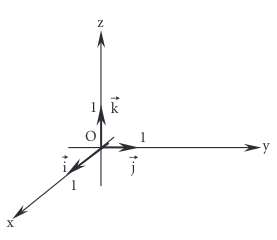
\includegraphics[width=0.5\textwidth]{./fig/fig1.53.png}
  \caption{Sistema de coordenadas no espaço}\label{fig:fig1.53}
\end{figure}

\subsection{Planos Coordenados}

Temos três planos coordenados (Figuras~\ref{fig:fig1.54a} e~\ref{fig:fig1.54b}):

\begin{itemize}
  \item Plano $xy$: $z=0$
  \item Plano $xz$: $y=0$
  \item Plano $yz$: $x=0$
\end{itemize}

\begin{figure}[H]
  \centering
  \begin{subfigure}
    \centering
    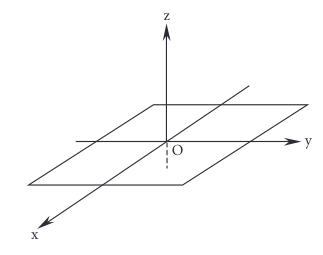
\includegraphics[width=0.5\linewidth]{./fig/fig1.54a.png}
    \caption{Plano $xy$}
    \label{fig:fig1.54a}
  \end{subfigure}
  \hfill
  \centering
  \begin{subfigure}
    \centering
    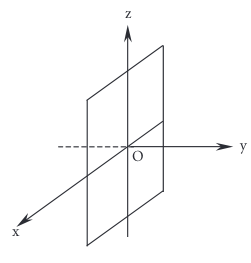
\includegraphics[width=0.5\linewidth]{./fig/fig1.54b.png}
    \caption{Plano $xz$}
    \label{fig:fig1.54b}
  \end{subfigure}
\end{figure}

\subsection{Representação de Vetores}

Para qualquer ponto $P(x,y,z)$, o vetor posição é:

\[
  \overrightarrow{OP} = x\vec{i} + y\vec{j} + z\vec{k} = (x,y,z)
\]

\begin{figure}[H]
  \centering
  \begin{subfigure}
    \centering
    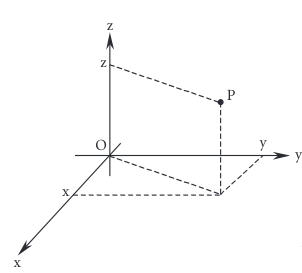
\includegraphics[width=0.5\linewidth]{./fig/fig1.55a.png}\label{fig:fig1.55a}
  \end{subfigure}
  \hfill
  \centering
  \begin{subfigure}
    \centering
    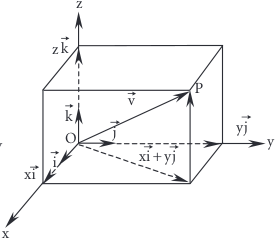
\includegraphics[width=0.5\linewidth]{./fig/fig1.55b.png}\label{fig:fig1.55b}
  \end{subfigure}
  \caption{Paralelepípedo e projeções}
\end{figure}

\subsection{Exemplos e Casos Especiais}

\begin{itemize}
  \item $2\vec{i} - 3\vec{j} + \vec{k} = (2,-3,1)$
  \item $-\vec{j} + 4\vec{k} = (0,-1,4)$
  \item Vetores canônicos: $\vec{i}=(1,0,0)$, $\vec{j}=(0,1,0)$,
    $\vec{k}=(0,0,1)$
\end{itemize}

\subsection{Localização de Pontos}

Para o paralelepípedo com $P(2,4,3)$ (Figura~\ref{fig:fig1.56}):

\begin{itemize}
  \item Eixo $x$: $A(2,0,0)$
  \item Eixo $y$: $C(0,4,0)$
  \item Eixo $z$: $E(0,0,3)$
  \item Plano $xy$: $B(2,4,0)$
  \item Plano $xz$: $F(2,0,3)$
  \item Plano $yz$: $D(0,4,3)$
\end{itemize}

\begin{figure}[H]
  \centering
  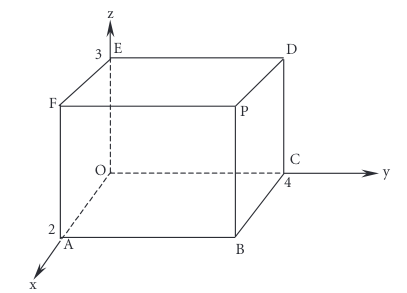
\includegraphics[width=0.5\textwidth]{./fig/fig1.56.png}
  \caption{Paralelepípedo e projeções}
  \label{fig:fig1.56}
\end{figure}

\subsection{Octantes}

O espaço é dividido em 8 octantes (Figura~\ref{fig:fig1.59}):

\begin{itemize}
  \item 1º octante: $(+,+,+)$
  \item 2º octante: $(-,+,+)$
  \item 3º octante: $(-,-,+)$
  \item 4º octante: $(+,-,+)$
  \item 5º octante: $(+,+,-)$
  \item 6º octante: $(-,+,-)$
  \item 7º octante: $(-,-,-)$
  \item 8º octante: $(+,-,-)$
\end{itemize}

\begin{figure}[H]
  \centering
  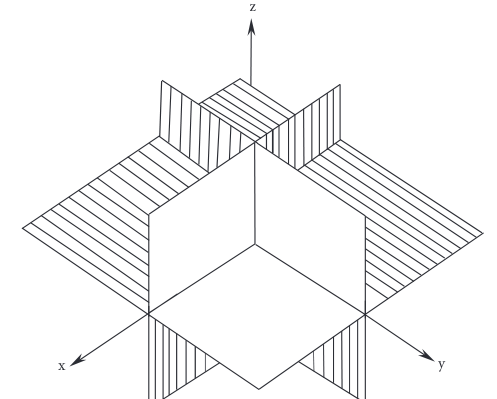
\includegraphics[width=0.6\textwidth]{./fig/fig1.59.png}
  \caption{Octantes do espaço}
  \label{fig:fig1.59}
\end{figure}

\subsection{Exemplos de Pontos}

\begin{itemize}
  \item Acima do plano $xy$ (cota $+2$):
    \begin{itemize}
      \item $A(6,4,2)$ - 1º octante
      \item $B(-5,3,2)$ - 2º octante
      \item $C(-6,-5,2)$ - 3º octante
      \item $D(5,-3,2)$ - 4º octante
    \end{itemize}

  \item Abaixo do plano $xy$ (cota $-2$):
    \begin{itemize}
      \item $A'(6,4,-2)$ - 5º octante
      \item $B'(-5,3,-2)$ - 6º octante
      \item $C'(-6,-5,-2)$ - 7º octante
      \item $D'(5,-3,-2)$ - 8º octante
    \end{itemize}
\end{itemize}

\begin{figure}[H]
  \centering
  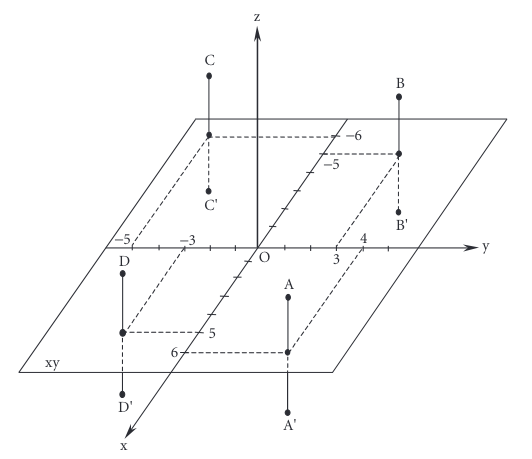
\includegraphics[width=0.7\textwidth]{./fig/fig1.60.png}
  \caption{Pontos em diferentes octantes}
  \label{fig:fig1.60}
\end{figure}

\subsection{Propriedades dos Vetores no Espaço}

As definições e conclusões no espaço são análogas às do plano:

\begin{enumerate}
  \item \textbf{Igualdade de vetores}: Dois vetores $\vec{u} = (x_1, y_1, z_1)$
    e $\vec{v} = (x_2, y_2, z_2)$ são iguais se, e somente se:
    \[
      x_1 = x_2, \quad y_1 = y_2 \quad \text{e} \quad z_1 = z_2
    \]

  \item \textbf{Operações básicas}: Para $\vec{u} = (x_1, y_1, z_1)$, $\vec{v} =
    (x_2, y_2, z_2)$ e $\alpha \in \mathbb{R}$:
    \[
      \vec{u} + \vec{v} = (x_1 + x_2, y_1 + y_2, z_1 + z_2)
    \]
    \[
      \alpha\vec{u} = (\alpha x_1, \alpha y_1, \alpha z_1)
    \]

  \item \textbf{Vetor definido por dois pontos}: Para $A(x_1,y_1,z_1)$ e
    $B(x_2,y_2,z_2)$:
    \[
      \overrightarrow{AB} = B - A = (x_2 - x_1, y_2 - y_1, z_2 - z_1)
    \]
    Se $\vec{v} = B - A$, então $B = A + \vec{v}$ (Figura~\ref{fig:fig1.61}).

    \begin{figure}[h]
      \centering
      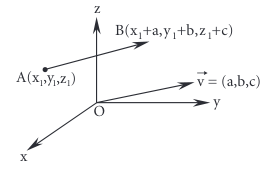
\includegraphics[width=0.4\textwidth]{./fig/fig1.61.png}
      \caption{Soma de ponto com vetor}\label{fig:fig1.61}
    \end{figure}

  \item \textbf{Ponto médio}: O ponto médio $M$ de $AB$ é:
    \[
      M\left(\frac{x_1+x_2}{2}, \frac{y_1+y_2}{2}, \frac{z_1+z_2}{2}\right)
    \]

  \item \textbf{Vetores paralelos}: Se $\vec{u} \parallel \vec{v}$, então:
    \[
      \vec{u} = \alpha\vec{v} \quad \text{ou} \quad \frac{x_1}{x_2} =
      \frac{y_1}{y_2} = \frac{z_1}{z_2}
    \]

  \item \textbf{Módulo de um vetor}: Para $\vec{v} = (x,y,z)$:
    \[
      |\vec{v}| = \sqrt{x^2 + y^2 + z^2}
    \]
    \textbf{Dedução:} O vetor $\vec{v} = (x, y, z)$ pode ser interpretado como
    um ponto no espaço tridimensional com coordenadas $(x, y, z)$, partindo da
    origem $(0,0,0)$. O módulo de $\vec{v}$ é a distância da origem até esse
    ponto.

    Utilizando a fórmula da distância euclidiana no $\mathbb{R}^3$, temos:
    \[
      |\vec{v}| = \sqrt{(x - 0)^2 + (y - 0)^2 + (z - 0)^2} = \sqrt{x^2 + y^2 +
      z^2}
    \]

    Portanto, o módulo de $\vec{v}$ é dado por:
    \[
      |\vec{v}| = \sqrt{x^2 + y^2 + z^2}
    \]
\end{enumerate}
